\documentclass[twoside]{book}

% Packages required by doxygen
\usepackage{fixltx2e}
\usepackage{calc}
\usepackage{doxygen}
\usepackage[export]{adjustbox} % also loads graphicx
\usepackage{graphicx}
\usepackage[utf8]{inputenc}
\usepackage{makeidx}
\usepackage{multicol}
\usepackage{multirow}
\PassOptionsToPackage{warn}{textcomp}
\usepackage{textcomp}
\usepackage[nointegrals]{wasysym}
\usepackage[table]{xcolor}

% Font selection
\usepackage[T1]{fontenc}
\usepackage[scaled=.90]{helvet}
\usepackage{courier}
\usepackage{amssymb}
\usepackage{sectsty}
\renewcommand{\familydefault}{\sfdefault}
\allsectionsfont{%
  \fontseries{bc}\selectfont%
  \color{darkgray}%
}
\renewcommand{\DoxyLabelFont}{%
  \fontseries{bc}\selectfont%
  \color{darkgray}%
}
\newcommand{\+}{\discretionary{\mbox{\scriptsize$\hookleftarrow$}}{}{}}

% Page & text layout
\usepackage{geometry}
\geometry{%
  a4paper,%
  top=2.5cm,%
  bottom=2.5cm,%
  left=2.5cm,%
  right=2.5cm%
}
\tolerance=750
\hfuzz=15pt
\hbadness=750
\setlength{\emergencystretch}{15pt}
\setlength{\parindent}{0cm}
\setlength{\parskip}{3ex plus 2ex minus 2ex}
\makeatletter
\renewcommand{\paragraph}{%
  \@startsection{paragraph}{4}{0ex}{-1.0ex}{1.0ex}{%
    \normalfont\normalsize\bfseries\SS@parafont%
  }%
}
\renewcommand{\subparagraph}{%
  \@startsection{subparagraph}{5}{0ex}{-1.0ex}{1.0ex}{%
    \normalfont\normalsize\bfseries\SS@subparafont%
  }%
}
\makeatother

% Headers & footers
\usepackage{fancyhdr}
\pagestyle{fancyplain}
\fancyhead[LE]{\fancyplain{}{\bfseries\thepage}}
\fancyhead[CE]{\fancyplain{}{}}
\fancyhead[RE]{\fancyplain{}{\bfseries\leftmark}}
\fancyhead[LO]{\fancyplain{}{\bfseries\rightmark}}
\fancyhead[CO]{\fancyplain{}{}}
\fancyhead[RO]{\fancyplain{}{\bfseries\thepage}}
\fancyfoot[LE]{\fancyplain{}{}}
\fancyfoot[CE]{\fancyplain{}{}}
\fancyfoot[RE]{\fancyplain{}{\bfseries\scriptsize Generated by Doxygen }}
\fancyfoot[LO]{\fancyplain{}{\bfseries\scriptsize Generated by Doxygen }}
\fancyfoot[CO]{\fancyplain{}{}}
\fancyfoot[RO]{\fancyplain{}{}}
\renewcommand{\footrulewidth}{0.4pt}
\renewcommand{\chaptermark}[1]{%
  \markboth{#1}{}%
}
\renewcommand{\sectionmark}[1]{%
  \markright{\thesection\ #1}%
}

% Indices & bibliography
\usepackage{natbib}
\usepackage[titles]{tocloft}
\setcounter{tocdepth}{3}
\setcounter{secnumdepth}{5}
\makeindex

% Hyperlinks (required, but should be loaded last)
\usepackage{ifpdf}
\ifpdf
  \usepackage[pdftex,pagebackref=true]{hyperref}
\else
  \usepackage[ps2pdf,pagebackref=true]{hyperref}
\fi
\hypersetup{%
  colorlinks=true,%
  linkcolor=blue,%
  citecolor=blue,%
  unicode%
}

% Custom commands
\newcommand{\clearemptydoublepage}{%
  \newpage{\pagestyle{empty}\cleardoublepage}%
}

\usepackage{caption}
\captionsetup{labelsep=space,justification=centering,font={bf},singlelinecheck=off,skip=4pt,position=top}

%===== C O N T E N T S =====

\begin{document}

% Titlepage & ToC
\hypersetup{pageanchor=false,
             bookmarksnumbered=true,
             pdfencoding=unicode
            }
\pagenumbering{roman}
\begin{titlepage}
\vspace*{7cm}
\begin{center}%
{\Large material\+\_\+handling\+\_\+robot }\\
\vspace*{1cm}
{\large Generated by Doxygen 1.8.11}\\
\end{center}
\end{titlepage}
\clearemptydoublepage
\tableofcontents
\clearemptydoublepage
\pagenumbering{arabic}
\hypersetup{pageanchor=true}

%--- Begin generated contents ---
\chapter{Class Index}
\section{Class List}
Here are the classes, structs, unions and interfaces with brief descriptions\+:\begin{DoxyCompactList}
\item\contentsline{section}{\hyperlink{classMaterialHandler}{Material\+Handler} \\*\hyperlink{classMaterialHandler}{Material\+Handler} class which has pickup and drop off locations as attributes, and has methods to get them }{\pageref{classMaterialHandler}}{}
\item\contentsline{section}{\hyperlink{classObstacleChange}{Obstacle\+Change} \\*\hyperlink{classObstacleChange}{Obstacle\+Change} class that spawns an object when robot arrives at location in gazebo and also has method that makes the object disappear }{\pageref{classObstacleChange}}{}
\item\contentsline{section}{\hyperlink{classPathPlanner}{Path\+Planner} \\*\hyperlink{classPathPlanner}{Path\+Planner} class that implements methods to send goal to move\+\_\+base package and also receive status, that indicates robot reached goal or not }{\pageref{classPathPlanner}}{}
\item\contentsline{section}{\hyperlink{structPosition}{Position} \\*A struct that stores position with x and y values indicating position of the object on the map }{\pageref{structPosition}}{}
\item\contentsline{section}{\hyperlink{classRobotController}{Robot\+Controller} \\*\hyperlink{classRobotController}{Robot\+Controller} class that subscribes to /raw\+\_\+cmd\+\_\+vel topic and remaps to /cmd\+\_\+vel topic }{\pageref{classRobotController}}{}
\end{DoxyCompactList}

\chapter{File Index}
\section{File List}
Here is a list of all documented files with brief descriptions\+:\begin{DoxyCompactList}
\item\contentsline{section}{/home/raja/material\+\_\+handling\+\_\+robot/include/material\+\_\+handling\+\_\+robot/{\bfseries Material\+Handler.\+h} }{\pageref{MaterialHandler_8h}}{}
\item\contentsline{section}{/home/raja/material\+\_\+handling\+\_\+robot/include/material\+\_\+handling\+\_\+robot/{\bfseries Obstacle\+Change.\+h} }{\pageref{ObstacleChange_8h}}{}
\item\contentsline{section}{/home/raja/material\+\_\+handling\+\_\+robot/include/material\+\_\+handling\+\_\+robot/{\bfseries Path\+Planner.\+h} }{\pageref{PathPlanner_8h}}{}
\item\contentsline{section}{/home/raja/material\+\_\+handling\+\_\+robot/include/material\+\_\+handling\+\_\+robot/{\bfseries Robot\+Controller.\+h} }{\pageref{RobotController_8h}}{}
\item\contentsline{section}{/home/raja/material\+\_\+handling\+\_\+robot/test/\hyperlink{ObstacleChangeTest_8cpp}{Obstacle\+Change\+Test.\+cpp} \\*Tests the member methods of \hyperlink{classObstacleChange}{Obstacle\+Change} class }{\pageref{ObstacleChangeTest_8cpp}}{}
\end{DoxyCompactList}

\chapter{Class Documentation}
\hypertarget{classMaterialHandler}{}\section{Material\+Handler Class Reference}
\label{classMaterialHandler}\index{Material\+Handler@{Material\+Handler}}


\hyperlink{classMaterialHandler}{Material\+Handler} class which has pickup and drop off locations as attributes, and has methods to get them.  




{\ttfamily \#include $<$Material\+Handler.\+h$>$}

\subsection*{Public Member Functions}
\begin{DoxyCompactItemize}
\item 
\hyperlink{classMaterialHandler_a1cb01a4bd9cad981ae5d3fdb7feda4e9}{Material\+Handler} ()
\item 
\hyperlink{classMaterialHandler_ad20121774c2dd6ef83a4749b8f012880}{$\sim$\+Material\+Handler} ()
\item 
\hyperlink{structPosition}{Position} \hyperlink{classMaterialHandler_aee5b970fe4ad65e965c8ca4bb406592f}{get\+Drop\+Off1} ()
\begin{DoxyCompactList}\small\item\em getter for drop\+Off\+Position1 which is a private attribute of this class. \end{DoxyCompactList}\item 
\hyperlink{structPosition}{Position} \hyperlink{classMaterialHandler_ad3d95f4e547213a07c79a87adcd02b70}{get\+Drop\+Off2} ()
\begin{DoxyCompactList}\small\item\em getter for drop\+Off\+Position2 which is a private attribute of this class. \end{DoxyCompactList}\item 
\hyperlink{structPosition}{Position} \hyperlink{classMaterialHandler_ad466acfc6d451eda3abfdb9380e5b9a8}{get\+Drop\+Off3} ()
\begin{DoxyCompactList}\small\item\em getter for drop\+Off\+Position3 which is a private attribute of this class. \end{DoxyCompactList}\item 
\hyperlink{structPosition}{Position} \hyperlink{classMaterialHandler_aa11e5fab9fc80e42f2f85ea8f016d7d3}{get\+Pick\+Up1} ()
\begin{DoxyCompactList}\small\item\em getter for pick\+Up\+Position1 which is a private attribute of this class. \end{DoxyCompactList}\item 
\hyperlink{structPosition}{Position} \hyperlink{classMaterialHandler_ab95a6ca4be40bd96fd23776398ff648e}{get\+Pick\+Up2} ()
\begin{DoxyCompactList}\small\item\em getter for pick\+Up\+Position2 which is a private attribute of this class. \end{DoxyCompactList}\item 
\hyperlink{structPosition}{Position} \hyperlink{classMaterialHandler_a4a88c1ea78485f756a909505ca003261}{get\+Pick\+Up3} ()
\begin{DoxyCompactList}\small\item\em getter for pick\+Up\+Position3 which is a private attribute of this class. \end{DoxyCompactList}\end{DoxyCompactItemize}


\subsection{Detailed Description}
\hyperlink{classMaterialHandler}{Material\+Handler} class which has pickup and drop off locations as attributes, and has methods to get them. 

\subsection{Constructor \& Destructor Documentation}
\index{Material\+Handler@{Material\+Handler}!Material\+Handler@{Material\+Handler}}
\index{Material\+Handler@{Material\+Handler}!Material\+Handler@{Material\+Handler}}
\subsubsection[{\texorpdfstring{Material\+Handler()}{MaterialHandler()}}]{\setlength{\rightskip}{0pt plus 5cm}Material\+Handler\+::\+Material\+Handler (
\begin{DoxyParamCaption}
{}
\end{DoxyParamCaption}
)}\hypertarget{classMaterialHandler_a1cb01a4bd9cad981ae5d3fdb7feda4e9}{}\label{classMaterialHandler_a1cb01a4bd9cad981ae5d3fdb7feda4e9}
constructor for this class.

constructor implementation for this class. \index{Material\+Handler@{Material\+Handler}!````~Material\+Handler@{$\sim$\+Material\+Handler}}
\index{````~Material\+Handler@{$\sim$\+Material\+Handler}!Material\+Handler@{Material\+Handler}}
\subsubsection[{\texorpdfstring{$\sim$\+Material\+Handler()}{~MaterialHandler()}}]{\setlength{\rightskip}{0pt plus 5cm}Material\+Handler\+::$\sim$\+Material\+Handler (
\begin{DoxyParamCaption}
{}
\end{DoxyParamCaption}
)}\hypertarget{classMaterialHandler_ad20121774c2dd6ef83a4749b8f012880}{}\label{classMaterialHandler_ad20121774c2dd6ef83a4749b8f012880}
Destructor for this class. 

\subsection{Member Function Documentation}
\index{Material\+Handler@{Material\+Handler}!get\+Drop\+Off1@{get\+Drop\+Off1}}
\index{get\+Drop\+Off1@{get\+Drop\+Off1}!Material\+Handler@{Material\+Handler}}
\subsubsection[{\texorpdfstring{get\+Drop\+Off1()}{getDropOff1()}}]{\setlength{\rightskip}{0pt plus 5cm}{\bf Position} Material\+Handler\+::get\+Drop\+Off1 (
\begin{DoxyParamCaption}
{}
\end{DoxyParamCaption}
)}\hypertarget{classMaterialHandler_aee5b970fe4ad65e965c8ca4bb406592f}{}\label{classMaterialHandler_aee5b970fe4ad65e965c8ca4bb406592f}


getter for drop\+Off\+Position1 which is a private attribute of this class. 


\begin{DoxyParams}{Parameters}
{\em None.} & \\
\hline
\end{DoxyParams}
\begin{DoxyReturn}{Returns}
struct \hyperlink{structPosition}{Position} returns a struct that has position of drop off 1 location. 
\end{DoxyReturn}
\index{Material\+Handler@{Material\+Handler}!get\+Drop\+Off2@{get\+Drop\+Off2}}
\index{get\+Drop\+Off2@{get\+Drop\+Off2}!Material\+Handler@{Material\+Handler}}
\subsubsection[{\texorpdfstring{get\+Drop\+Off2()}{getDropOff2()}}]{\setlength{\rightskip}{0pt plus 5cm}{\bf Position} Material\+Handler\+::get\+Drop\+Off2 (
\begin{DoxyParamCaption}
{}
\end{DoxyParamCaption}
)}\hypertarget{classMaterialHandler_ad3d95f4e547213a07c79a87adcd02b70}{}\label{classMaterialHandler_ad3d95f4e547213a07c79a87adcd02b70}


getter for drop\+Off\+Position2 which is a private attribute of this class. 


\begin{DoxyParams}{Parameters}
{\em None.} & \\
\hline
\end{DoxyParams}
\begin{DoxyReturn}{Returns}
struct \hyperlink{structPosition}{Position} returns a struct that has position of drop off 2 location. 
\end{DoxyReturn}
\index{Material\+Handler@{Material\+Handler}!get\+Drop\+Off3@{get\+Drop\+Off3}}
\index{get\+Drop\+Off3@{get\+Drop\+Off3}!Material\+Handler@{Material\+Handler}}
\subsubsection[{\texorpdfstring{get\+Drop\+Off3()}{getDropOff3()}}]{\setlength{\rightskip}{0pt plus 5cm}{\bf Position} Material\+Handler\+::get\+Drop\+Off3 (
\begin{DoxyParamCaption}
{}
\end{DoxyParamCaption}
)}\hypertarget{classMaterialHandler_ad466acfc6d451eda3abfdb9380e5b9a8}{}\label{classMaterialHandler_ad466acfc6d451eda3abfdb9380e5b9a8}


getter for drop\+Off\+Position3 which is a private attribute of this class. 


\begin{DoxyParams}{Parameters}
{\em None.} & \\
\hline
\end{DoxyParams}
\begin{DoxyReturn}{Returns}
struct \hyperlink{structPosition}{Position} returns a struct that has position of drop off 3 location. 
\end{DoxyReturn}
\index{Material\+Handler@{Material\+Handler}!get\+Pick\+Up1@{get\+Pick\+Up1}}
\index{get\+Pick\+Up1@{get\+Pick\+Up1}!Material\+Handler@{Material\+Handler}}
\subsubsection[{\texorpdfstring{get\+Pick\+Up1()}{getPickUp1()}}]{\setlength{\rightskip}{0pt plus 5cm}{\bf Position} Material\+Handler\+::get\+Pick\+Up1 (
\begin{DoxyParamCaption}
{}
\end{DoxyParamCaption}
)}\hypertarget{classMaterialHandler_aa11e5fab9fc80e42f2f85ea8f016d7d3}{}\label{classMaterialHandler_aa11e5fab9fc80e42f2f85ea8f016d7d3}


getter for pick\+Up\+Position1 which is a private attribute of this class. 


\begin{DoxyParams}{Parameters}
{\em None.} & \\
\hline
\end{DoxyParams}
\begin{DoxyReturn}{Returns}
struct \hyperlink{structPosition}{Position} returns a struct that has position of pickup 1 location. 
\end{DoxyReturn}
\index{Material\+Handler@{Material\+Handler}!get\+Pick\+Up2@{get\+Pick\+Up2}}
\index{get\+Pick\+Up2@{get\+Pick\+Up2}!Material\+Handler@{Material\+Handler}}
\subsubsection[{\texorpdfstring{get\+Pick\+Up2()}{getPickUp2()}}]{\setlength{\rightskip}{0pt plus 5cm}{\bf Position} Material\+Handler\+::get\+Pick\+Up2 (
\begin{DoxyParamCaption}
{}
\end{DoxyParamCaption}
)}\hypertarget{classMaterialHandler_ab95a6ca4be40bd96fd23776398ff648e}{}\label{classMaterialHandler_ab95a6ca4be40bd96fd23776398ff648e}


getter for pick\+Up\+Position2 which is a private attribute of this class. 


\begin{DoxyParams}{Parameters}
{\em None.} & \\
\hline
\end{DoxyParams}
\begin{DoxyReturn}{Returns}
struct \hyperlink{structPosition}{Position} returns a struct that has position of pickup 2 location. 
\end{DoxyReturn}
\index{Material\+Handler@{Material\+Handler}!get\+Pick\+Up3@{get\+Pick\+Up3}}
\index{get\+Pick\+Up3@{get\+Pick\+Up3}!Material\+Handler@{Material\+Handler}}
\subsubsection[{\texorpdfstring{get\+Pick\+Up3()}{getPickUp3()}}]{\setlength{\rightskip}{0pt plus 5cm}{\bf Position} Material\+Handler\+::get\+Pick\+Up3 (
\begin{DoxyParamCaption}
{}
\end{DoxyParamCaption}
)}\hypertarget{classMaterialHandler_a4a88c1ea78485f756a909505ca003261}{}\label{classMaterialHandler_a4a88c1ea78485f756a909505ca003261}


getter for pick\+Up\+Position3 which is a private attribute of this class. 


\begin{DoxyParams}{Parameters}
{\em None.} & \\
\hline
\end{DoxyParams}
\begin{DoxyReturn}{Returns}
struct \hyperlink{structPosition}{Position} returns a struct that has position of pickup 3 location. 
\end{DoxyReturn}


The documentation for this class was generated from the following files\+:\begin{DoxyCompactItemize}
\item 
include/material\+\_\+handling\+\_\+robot/\hyperlink{MaterialHandler_8h}{Material\+Handler.\+h}\item 
src/\hyperlink{MaterialHandler_8cpp}{Material\+Handler.\+cpp}\end{DoxyCompactItemize}

\hypertarget{classObstacleChange}{}\section{Obstacle\+Change Class Reference}
\label{classObstacleChange}\index{Obstacle\+Change@{Obstacle\+Change}}


\hyperlink{classObstacleChange}{Obstacle\+Change} class that spawns an object when robot arrives at location in gazebo and also has method that makes the object disappear.  




{\ttfamily \#include $<$Obstacle\+Change.\+h$>$}

\subsection*{Public Member Functions}
\begin{DoxyCompactItemize}
\item 
\hyperlink{classObstacleChange_a57f5c3efb9d59055477b82576393ae3a}{Obstacle\+Change} ()
\item 
\hyperlink{classObstacleChange_a7660d8cc43e71263870ac6d3558dc208}{$\sim$\+Obstacle\+Change} ()
\item 
std\+::string \hyperlink{classObstacleChange_a3a50e08dfade39833a7c3322d8f083a6}{set\+Target\+Point} (double target\+Point)
\begin{DoxyCompactList}\small\item\em sets the string for the target point. \end{DoxyCompactList}\item 
std\+::string \hyperlink{classObstacleChange_acd201b19981248a932a73f6ee892aea4}{spawn\+Object} (double x, double y)
\begin{DoxyCompactList}\small\item\em spawns a wooden block in gazebo at location x, y specified. \end{DoxyCompactList}\item 
std\+::string \hyperlink{classObstacleChange_a3aee4006b737cd0dd52b8c44fdcbd0e1}{destroy\+Object} ()
\begin{DoxyCompactList}\small\item\em destroys the spawned object indicating robot picked up the object. \end{DoxyCompactList}\end{DoxyCompactItemize}


\subsection{Detailed Description}
\hyperlink{classObstacleChange}{Obstacle\+Change} class that spawns an object when robot arrives at location in gazebo and also has method that makes the object disappear. 

M\+IT License

Copyright (c) 2019 Vamshi Bogoju, Raja Srinivas Iskala

Permission is hereby granted, free of charge, to any person obtaining a copy of this software and associated documentation files (the \char`\"{}\+Software\char`\"{}), to deal in the Software without restriction, including without limitation the rights to use, copy, modify, merge, publish, distribute, sublicense, and/or sell copies of the Software, and to permit persons to whom the Software is furnished to do so, subject to the following conditions\+:

The above copyright notice and this permission notice shall be included in all copies or substantial portions of the Software.

T\+HE S\+O\+F\+T\+W\+A\+RE IS P\+R\+O\+V\+I\+D\+ED \char`\"{}\+A\+S I\+S\char`\"{}, W\+I\+T\+H\+O\+UT W\+A\+R\+R\+A\+N\+TY OF A\+NY K\+I\+ND, E\+X\+P\+R\+E\+SS OR I\+M\+P\+L\+I\+ED, I\+N\+C\+L\+U\+D\+I\+NG B\+UT N\+OT L\+I\+M\+I\+T\+ED TO T\+HE W\+A\+R\+R\+A\+N\+T\+I\+ES OF M\+E\+R\+C\+H\+A\+N\+T\+A\+B\+I\+L\+I\+TY, F\+I\+T\+N\+E\+SS F\+OR A P\+A\+R\+T\+I\+C\+U\+L\+AR P\+U\+R\+P\+O\+SE A\+ND N\+O\+N\+I\+N\+F\+R\+I\+N\+G\+E\+M\+E\+NT. IN NO E\+V\+E\+NT S\+H\+A\+LL T\+HE A\+U\+T\+H\+O\+RS OR C\+O\+P\+Y\+R\+I\+G\+HT H\+O\+L\+D\+E\+RS BE L\+I\+A\+B\+LE F\+OR A\+NY C\+L\+A\+IM, D\+A\+M\+A\+G\+ES OR O\+T\+H\+ER L\+I\+A\+B\+I\+L\+I\+TY, W\+H\+E\+T\+H\+ER IN AN A\+C\+T\+I\+ON OF C\+O\+N\+T\+R\+A\+CT, T\+O\+RT OR O\+T\+H\+E\+R\+W\+I\+SE, A\+R\+I\+S\+I\+NG F\+R\+OM, O\+UT OF OR IN C\+O\+N\+N\+E\+C\+T\+I\+ON W\+I\+TH T\+HE S\+O\+F\+T\+W\+A\+RE OR T\+HE U\+SE OR O\+T\+H\+ER D\+E\+A\+L\+I\+N\+GS IN T\+HE S\+O\+F\+T\+W\+A\+RE. 

\subsection{Constructor \& Destructor Documentation}
\index{Obstacle\+Change@{Obstacle\+Change}!Obstacle\+Change@{Obstacle\+Change}}
\index{Obstacle\+Change@{Obstacle\+Change}!Obstacle\+Change@{Obstacle\+Change}}
\subsubsection[{\texorpdfstring{Obstacle\+Change()}{ObstacleChange()}}]{\setlength{\rightskip}{0pt plus 5cm}Obstacle\+Change\+::\+Obstacle\+Change (
\begin{DoxyParamCaption}
{}
\end{DoxyParamCaption}
)}\hypertarget{classObstacleChange_a57f5c3efb9d59055477b82576393ae3a}{}\label{classObstacleChange_a57f5c3efb9d59055477b82576393ae3a}
constructor for this class.

M\+IT License

Copyright (c) 2019 Vamshi Bogoju, Raja Srinivas Iskala

Permission is hereby granted, free of charge, to any person obtaining a copy of this software and associated documentation files (the \char`\"{}\+Software\char`\"{}), to deal in the Software without restriction, including without limitation the rights to use, copy, modify, merge, publish, distribute, sublicense, and/or sell copies of the Software, and to permit persons to whom the Software is furnished to do so, subject to the following conditions\+:

The above copyright notice and this permission notice shall be included in all copies or substantial portions of the Software.

T\+HE S\+O\+F\+T\+W\+A\+RE IS P\+R\+O\+V\+I\+D\+ED \char`\"{}\+A\+S I\+S\char`\"{}, W\+I\+T\+H\+O\+UT W\+A\+R\+R\+A\+N\+TY OF A\+NY K\+I\+ND, E\+X\+P\+R\+E\+SS OR I\+M\+P\+L\+I\+ED, I\+N\+C\+L\+U\+D\+I\+NG B\+UT N\+OT L\+I\+M\+I\+T\+ED TO T\+HE W\+A\+R\+R\+A\+N\+T\+I\+ES OF M\+E\+R\+C\+H\+A\+N\+T\+A\+B\+I\+L\+I\+TY, F\+I\+T\+N\+E\+SS F\+OR A P\+A\+R\+T\+I\+C\+U\+L\+AR P\+U\+R\+P\+O\+SE A\+ND N\+O\+N\+I\+N\+F\+R\+I\+N\+G\+E\+M\+E\+NT. IN NO E\+V\+E\+NT S\+H\+A\+LL T\+HE A\+U\+T\+H\+O\+RS OR C\+O\+P\+Y\+R\+I\+G\+HT H\+O\+L\+D\+E\+RS BE L\+I\+A\+B\+LE F\+OR A\+NY C\+L\+A\+IM, D\+A\+M\+A\+G\+ES OR O\+T\+H\+ER L\+I\+A\+B\+I\+L\+I\+TY, W\+H\+E\+T\+H\+ER IN AN A\+C\+T\+I\+ON OF C\+O\+N\+T\+R\+A\+CT, T\+O\+RT OR O\+T\+H\+E\+R\+W\+I\+SE, A\+R\+I\+S\+I\+NG F\+R\+OM, O\+UT OF OR IN C\+O\+N\+N\+E\+C\+T\+I\+ON W\+I\+TH T\+HE S\+O\+F\+T\+W\+A\+RE OR T\+HE U\+SE OR O\+T\+H\+ER D\+E\+A\+L\+I\+N\+GS IN T\+HE S\+O\+F\+T\+W\+A\+RE. \index{Obstacle\+Change@{Obstacle\+Change}!````~Obstacle\+Change@{$\sim$\+Obstacle\+Change}}
\index{````~Obstacle\+Change@{$\sim$\+Obstacle\+Change}!Obstacle\+Change@{Obstacle\+Change}}
\subsubsection[{\texorpdfstring{$\sim$\+Obstacle\+Change()}{~ObstacleChange()}}]{\setlength{\rightskip}{0pt plus 5cm}Obstacle\+Change\+::$\sim$\+Obstacle\+Change (
\begin{DoxyParamCaption}
{}
\end{DoxyParamCaption}
)}\hypertarget{classObstacleChange_a7660d8cc43e71263870ac6d3558dc208}{}\label{classObstacleChange_a7660d8cc43e71263870ac6d3558dc208}
Destructor for this class. 

\subsection{Member Function Documentation}
\index{Obstacle\+Change@{Obstacle\+Change}!destroy\+Object@{destroy\+Object}}
\index{destroy\+Object@{destroy\+Object}!Obstacle\+Change@{Obstacle\+Change}}
\subsubsection[{\texorpdfstring{destroy\+Object()}{destroyObject()}}]{\setlength{\rightskip}{0pt plus 5cm}std\+::string Obstacle\+Change\+::destroy\+Object (
\begin{DoxyParamCaption}
{}
\end{DoxyParamCaption}
)}\hypertarget{classObstacleChange_a3aee4006b737cd0dd52b8c44fdcbd0e1}{}\label{classObstacleChange_a3aee4006b737cd0dd52b8c44fdcbd0e1}


destroys the spawned object indicating robot picked up the object. 


\begin{DoxyParams}{Parameters}
{\em None} & \\
\hline
\end{DoxyParams}
\begin{DoxyReturn}{Returns}
std\+::string 
\end{DoxyReturn}
\index{Obstacle\+Change@{Obstacle\+Change}!set\+Target\+Point@{set\+Target\+Point}}
\index{set\+Target\+Point@{set\+Target\+Point}!Obstacle\+Change@{Obstacle\+Change}}
\subsubsection[{\texorpdfstring{set\+Target\+Point(double target\+Point)}{setTargetPoint(double targetPoint)}}]{\setlength{\rightskip}{0pt plus 5cm}std\+::string Obstacle\+Change\+::set\+Target\+Point (
\begin{DoxyParamCaption}
\item[{double}]{target\+Point}
\end{DoxyParamCaption}
)}\hypertarget{classObstacleChange_a3a50e08dfade39833a7c3322d8f083a6}{}\label{classObstacleChange_a3a50e08dfade39833a7c3322d8f083a6}


sets the string for the target point. 


\begin{DoxyParams}{Parameters}
{\em double} & target\+Point. \\
\hline
\end{DoxyParams}
\begin{DoxyReturn}{Returns}
std\+::string 
\end{DoxyReturn}
\index{Obstacle\+Change@{Obstacle\+Change}!spawn\+Object@{spawn\+Object}}
\index{spawn\+Object@{spawn\+Object}!Obstacle\+Change@{Obstacle\+Change}}
\subsubsection[{\texorpdfstring{spawn\+Object(double x, double y)}{spawnObject(double x, double y)}}]{\setlength{\rightskip}{0pt plus 5cm}std\+::string Obstacle\+Change\+::spawn\+Object (
\begin{DoxyParamCaption}
\item[{double}]{x, }
\item[{double}]{y}
\end{DoxyParamCaption}
)}\hypertarget{classObstacleChange_acd201b19981248a932a73f6ee892aea4}{}\label{classObstacleChange_acd201b19981248a932a73f6ee892aea4}


spawns a wooden block in gazebo at location x, y specified. 


\begin{DoxyParams}{Parameters}
{\em double} & x which is x position on the map where the model to spawns. \\
\hline
{\em double} & y which is y position on the map where the model to spawns. \\
\hline
\end{DoxyParams}
\begin{DoxyReturn}{Returns}
std\+::string 
\end{DoxyReturn}


The documentation for this class was generated from the following files\+:\begin{DoxyCompactItemize}
\item 
include/material\+\_\+handling\+\_\+robot/Obstacle\+Change.\+h\item 
src/Obstacle\+Change.\+cpp\end{DoxyCompactItemize}

\hypertarget{classPathPlanner}{}\section{Path\+Planner Class Reference}
\label{classPathPlanner}\index{Path\+Planner@{Path\+Planner}}


\hyperlink{classPathPlanner}{Path\+Planner} class that implements methods to send goal to move\+\_\+base package and also receive status, that indicates robot reached goal or not.  




{\ttfamily \#include $<$Path\+Planner.\+h$>$}

\subsection*{Public Member Functions}
\begin{DoxyCompactItemize}
\item 
\hyperlink{classPathPlanner_a376f30d795cfe0a40f8923f49336f7da}{Path\+Planner} ()
\item 
\hyperlink{classPathPlanner_a61bd61f848e519df56b75eddd3732ab8}{$\sim$\+Path\+Planner} ()
\item 
void \hyperlink{classPathPlanner_a3143ffa68678f4f30917565c339802dc}{set\+Goal} (double x, double y)
\begin{DoxyCompactList}\small\item\em sets the goal which is a private attribute to this class of type move\+\_\+base\+\_\+msgs\+::\+Move\+Base\+Action\+Goal \end{DoxyCompactList}\item 
move\+\_\+base\+\_\+msgs\+::\+Move\+Base\+Action\+Goal \hyperlink{classPathPlanner_a5828b4927eb0a4c4ab64d134ae6fbf3a}{get\+Goal} ()
\begin{DoxyCompactList}\small\item\em gets the goal that is being published, getter for private data member. \end{DoxyCompactList}\item 
void \hyperlink{classPathPlanner_a32ee3e597aace449eb1c2e2a7ff44439}{send\+Goal} ()
\begin{DoxyCompactList}\small\item\em A publisher that sends the goal to move\+\_\+base node by publishing to /move\+\_\+base/goal topic. \end{DoxyCompactList}\item 
uint8\+\_\+t \hyperlink{classPathPlanner_af2e19a41d18a7071f64c2973f1758c97}{get\+Status} ()
\begin{DoxyCompactList}\small\item\em A getter that gets the status of the robot currently helpful in tracking the progree of robot motion. \end{DoxyCompactList}\item 
void \hyperlink{classPathPlanner_a75b2efc17fc0d73a74de77bece725b3e}{subscribe\+Status} ()
\begin{DoxyCompactList}\small\item\em A subscriber to \char`\"{}/move\+\_\+base/status\char`\"{} topic which is helpful to get status. \end{DoxyCompactList}\item 
void \hyperlink{classPathPlanner_afa6a07572c40c98be76b19f592e8267d}{reached\+Target\+Callback} (const actionlib\+\_\+msgs\+::\+Goal\+Status\+Array\+::\+Const\+Ptr \&msg)
\begin{DoxyCompactList}\small\item\em A callback function for status subscriber, this method retrieves current status of the robot and stores in variable. \end{DoxyCompactList}\end{DoxyCompactItemize}


\subsection{Detailed Description}
\hyperlink{classPathPlanner}{Path\+Planner} class that implements methods to send goal to move\+\_\+base package and also receive status, that indicates robot reached goal or not. 

M\+IT License

Copyright (c) 2019 Vamshi Bogoju, Raja Srinivas Iskala

Permission is hereby granted, free of charge, to any person obtaining a copy of this software and associated documentation files (the \char`\"{}\+Software\char`\"{}), to deal in the Software without restriction, including without limitation the rights to use, copy, modify, merge, publish, distribute, sublicense, and/or sell copies of the Software, and to permit persons to whom the Software is furnished to do so, subject to the following conditions\+:

The above copyright notice and this permission notice shall be included in all copies or substantial portions of the Software.

T\+HE S\+O\+F\+T\+W\+A\+RE IS P\+R\+O\+V\+I\+D\+ED \char`\"{}\+A\+S I\+S\char`\"{}, W\+I\+T\+H\+O\+UT W\+A\+R\+R\+A\+N\+TY OF A\+NY K\+I\+ND, E\+X\+P\+R\+E\+SS OR I\+M\+P\+L\+I\+ED, I\+N\+C\+L\+U\+D\+I\+NG B\+UT N\+OT L\+I\+M\+I\+T\+ED TO T\+HE W\+A\+R\+R\+A\+N\+T\+I\+ES OF M\+E\+R\+C\+H\+A\+N\+T\+A\+B\+I\+L\+I\+TY, F\+I\+T\+N\+E\+SS F\+OR A P\+A\+R\+T\+I\+C\+U\+L\+AR P\+U\+R\+P\+O\+SE A\+ND N\+O\+N\+I\+N\+F\+R\+I\+N\+G\+E\+M\+E\+NT. IN NO E\+V\+E\+NT S\+H\+A\+LL T\+HE A\+U\+T\+H\+O\+RS OR C\+O\+P\+Y\+R\+I\+G\+HT H\+O\+L\+D\+E\+RS BE L\+I\+A\+B\+LE F\+OR A\+NY C\+L\+A\+IM, D\+A\+M\+A\+G\+ES OR O\+T\+H\+ER L\+I\+A\+B\+I\+L\+I\+TY, W\+H\+E\+T\+H\+ER IN AN A\+C\+T\+I\+ON OF C\+O\+N\+T\+R\+A\+CT, T\+O\+RT OR O\+T\+H\+E\+R\+W\+I\+SE, A\+R\+I\+S\+I\+NG F\+R\+OM, O\+UT OF OR IN C\+O\+N\+N\+E\+C\+T\+I\+ON W\+I\+TH T\+HE S\+O\+F\+T\+W\+A\+RE OR T\+HE U\+SE OR O\+T\+H\+ER D\+E\+A\+L\+I\+N\+GS IN T\+HE S\+O\+F\+T\+W\+A\+RE. 

\subsection{Constructor \& Destructor Documentation}
\index{Path\+Planner@{Path\+Planner}!Path\+Planner@{Path\+Planner}}
\index{Path\+Planner@{Path\+Planner}!Path\+Planner@{Path\+Planner}}
\subsubsection[{\texorpdfstring{Path\+Planner()}{PathPlanner()}}]{\setlength{\rightskip}{0pt plus 5cm}Path\+Planner\+::\+Path\+Planner (
\begin{DoxyParamCaption}
{}
\end{DoxyParamCaption}
)}\hypertarget{classPathPlanner_a376f30d795cfe0a40f8923f49336f7da}{}\label{classPathPlanner_a376f30d795cfe0a40f8923f49336f7da}
constructor for this class.

M\+IT License

Copyright (c) 2019 Vamshi Bogoju, Raja Srinivas Iskala

Permission is hereby granted, free of charge, to any person obtaining a copy of this software and associated documentation files (the \char`\"{}\+Software\char`\"{}), to deal in the Software without restriction, including without limitation the rights to use, copy, modify, merge, publish, distribute, sublicense, and/or sell copies of the Software, and to permit persons to whom the Software is furnished to do so, subject to the following conditions\+:

The above copyright notice and this permission notice shall be included in all copies or substantial portions of the Software.

T\+HE S\+O\+F\+T\+W\+A\+RE IS P\+R\+O\+V\+I\+D\+ED \char`\"{}\+A\+S I\+S\char`\"{}, W\+I\+T\+H\+O\+UT W\+A\+R\+R\+A\+N\+TY OF A\+NY K\+I\+ND, E\+X\+P\+R\+E\+SS OR I\+M\+P\+L\+I\+ED, I\+N\+C\+L\+U\+D\+I\+NG B\+UT N\+OT L\+I\+M\+I\+T\+ED TO T\+HE W\+A\+R\+R\+A\+N\+T\+I\+ES OF M\+E\+R\+C\+H\+A\+N\+T\+A\+B\+I\+L\+I\+TY, F\+I\+T\+N\+E\+SS F\+OR A P\+A\+R\+T\+I\+C\+U\+L\+AR P\+U\+R\+P\+O\+SE A\+ND N\+O\+N\+I\+N\+F\+R\+I\+N\+G\+E\+M\+E\+NT. IN NO E\+V\+E\+NT S\+H\+A\+LL T\+HE A\+U\+T\+H\+O\+RS OR C\+O\+P\+Y\+R\+I\+G\+HT H\+O\+L\+D\+E\+RS BE L\+I\+A\+B\+LE F\+OR A\+NY C\+L\+A\+IM, D\+A\+M\+A\+G\+ES OR O\+T\+H\+ER L\+I\+A\+B\+I\+L\+I\+TY, W\+H\+E\+T\+H\+ER IN AN A\+C\+T\+I\+ON OF C\+O\+N\+T\+R\+A\+CT, T\+O\+RT OR O\+T\+H\+E\+R\+W\+I\+SE, A\+R\+I\+S\+I\+NG F\+R\+OM, O\+UT OF OR IN C\+O\+N\+N\+E\+C\+T\+I\+ON W\+I\+TH T\+HE S\+O\+F\+T\+W\+A\+RE OR T\+HE U\+SE OR O\+T\+H\+ER D\+E\+A\+L\+I\+N\+GS IN T\+HE S\+O\+F\+T\+W\+A\+RE. \index{Path\+Planner@{Path\+Planner}!````~Path\+Planner@{$\sim$\+Path\+Planner}}
\index{````~Path\+Planner@{$\sim$\+Path\+Planner}!Path\+Planner@{Path\+Planner}}
\subsubsection[{\texorpdfstring{$\sim$\+Path\+Planner()}{~PathPlanner()}}]{\setlength{\rightskip}{0pt plus 5cm}Path\+Planner\+::$\sim$\+Path\+Planner (
\begin{DoxyParamCaption}
{}
\end{DoxyParamCaption}
)}\hypertarget{classPathPlanner_a61bd61f848e519df56b75eddd3732ab8}{}\label{classPathPlanner_a61bd61f848e519df56b75eddd3732ab8}
Detructor for this class. 

\subsection{Member Function Documentation}
\index{Path\+Planner@{Path\+Planner}!get\+Goal@{get\+Goal}}
\index{get\+Goal@{get\+Goal}!Path\+Planner@{Path\+Planner}}
\subsubsection[{\texorpdfstring{get\+Goal()}{getGoal()}}]{\setlength{\rightskip}{0pt plus 5cm}move\+\_\+base\+\_\+msgs\+::\+Move\+Base\+Action\+Goal Path\+Planner\+::get\+Goal (
\begin{DoxyParamCaption}
{}
\end{DoxyParamCaption}
)}\hypertarget{classPathPlanner_a5828b4927eb0a4c4ab64d134ae6fbf3a}{}\label{classPathPlanner_a5828b4927eb0a4c4ab64d134ae6fbf3a}


gets the goal that is being published, getter for private data member. 


\begin{DoxyParams}{Parameters}
{\em None.} & \\
\hline
\end{DoxyParams}
\begin{DoxyReturn}{Returns}
move\+\_\+base\+\_\+msgs\+::\+Move\+Base\+Action\+Goal returns goal position. 
\end{DoxyReturn}
\index{Path\+Planner@{Path\+Planner}!get\+Status@{get\+Status}}
\index{get\+Status@{get\+Status}!Path\+Planner@{Path\+Planner}}
\subsubsection[{\texorpdfstring{get\+Status()}{getStatus()}}]{\setlength{\rightskip}{0pt plus 5cm}uint8\+\_\+t Path\+Planner\+::get\+Status (
\begin{DoxyParamCaption}
{}
\end{DoxyParamCaption}
)}\hypertarget{classPathPlanner_af2e19a41d18a7071f64c2973f1758c97}{}\label{classPathPlanner_af2e19a41d18a7071f64c2973f1758c97}


A getter that gets the status of the robot currently helpful in tracking the progree of robot motion. 


\begin{DoxyParams}{Parameters}
{\em None.} & \\
\hline
\end{DoxyParams}
\begin{DoxyReturn}{Returns}
uint8\+\_\+t returns the status variable stored in the actionlib\+\_\+msgs\+::\+Goal\+Status\+Array message. 
\end{DoxyReturn}
\index{Path\+Planner@{Path\+Planner}!reached\+Target\+Callback@{reached\+Target\+Callback}}
\index{reached\+Target\+Callback@{reached\+Target\+Callback}!Path\+Planner@{Path\+Planner}}
\subsubsection[{\texorpdfstring{reached\+Target\+Callback(const actionlib\+\_\+msgs\+::\+Goal\+Status\+Array\+::\+Const\+Ptr \&msg)}{reachedTargetCallback(const actionlib_msgs::GoalStatusArray::ConstPtr &msg)}}]{\setlength{\rightskip}{0pt plus 5cm}void Path\+Planner\+::reached\+Target\+Callback (
\begin{DoxyParamCaption}
\item[{const actionlib\+\_\+msgs\+::\+Goal\+Status\+Array\+::\+Const\+Ptr \&}]{msg}
\end{DoxyParamCaption}
)}\hypertarget{classPathPlanner_afa6a07572c40c98be76b19f592e8267d}{}\label{classPathPlanner_afa6a07572c40c98be76b19f592e8267d}


A callback function for status subscriber, this method retrieves current status of the robot and stores in variable. 


\begin{DoxyParams}{Parameters}
{\em actionlib\+\_\+msgs\+::\+Goal\+Status\+Array\+::\+Const\+Ptr\&} & msg A pointer to a message type that has status information. \\
\hline
\end{DoxyParams}
\begin{DoxyReturn}{Returns}
None. 
\end{DoxyReturn}
\index{Path\+Planner@{Path\+Planner}!send\+Goal@{send\+Goal}}
\index{send\+Goal@{send\+Goal}!Path\+Planner@{Path\+Planner}}
\subsubsection[{\texorpdfstring{send\+Goal()}{sendGoal()}}]{\setlength{\rightskip}{0pt plus 5cm}void Path\+Planner\+::send\+Goal (
\begin{DoxyParamCaption}
{}
\end{DoxyParamCaption}
)}\hypertarget{classPathPlanner_a32ee3e597aace449eb1c2e2a7ff44439}{}\label{classPathPlanner_a32ee3e597aace449eb1c2e2a7ff44439}


A publisher that sends the goal to move\+\_\+base node by publishing to /move\+\_\+base/goal topic. 


\begin{DoxyParams}{Parameters}
{\em None.} & \\
\hline
\end{DoxyParams}
\begin{DoxyReturn}{Returns}
None 
\end{DoxyReturn}
\index{Path\+Planner@{Path\+Planner}!set\+Goal@{set\+Goal}}
\index{set\+Goal@{set\+Goal}!Path\+Planner@{Path\+Planner}}
\subsubsection[{\texorpdfstring{set\+Goal(double x, double y)}{setGoal(double x, double y)}}]{\setlength{\rightskip}{0pt plus 5cm}void Path\+Planner\+::set\+Goal (
\begin{DoxyParamCaption}
\item[{double}]{x, }
\item[{double}]{y}
\end{DoxyParamCaption}
)}\hypertarget{classPathPlanner_a3143ffa68678f4f30917565c339802dc}{}\label{classPathPlanner_a3143ffa68678f4f30917565c339802dc}


sets the goal which is a private attribute to this class of type move\+\_\+base\+\_\+msgs\+::\+Move\+Base\+Action\+Goal 


\begin{DoxyParams}{Parameters}
{\em double} & x which is x position of the goal that is sent. \\
\hline
{\em double} & y which is y position of the goal that is sent. \\
\hline
\end{DoxyParams}
\begin{DoxyReturn}{Returns}
None 
\end{DoxyReturn}
\index{Path\+Planner@{Path\+Planner}!subscribe\+Status@{subscribe\+Status}}
\index{subscribe\+Status@{subscribe\+Status}!Path\+Planner@{Path\+Planner}}
\subsubsection[{\texorpdfstring{subscribe\+Status()}{subscribeStatus()}}]{\setlength{\rightskip}{0pt plus 5cm}void Path\+Planner\+::subscribe\+Status (
\begin{DoxyParamCaption}
{}
\end{DoxyParamCaption}
)}\hypertarget{classPathPlanner_a75b2efc17fc0d73a74de77bece725b3e}{}\label{classPathPlanner_a75b2efc17fc0d73a74de77bece725b3e}


A subscriber to \char`\"{}/move\+\_\+base/status\char`\"{} topic which is helpful to get status. 


\begin{DoxyParams}{Parameters}
{\em None.} & \\
\hline
\end{DoxyParams}
\begin{DoxyReturn}{Returns}
None. 
\end{DoxyReturn}


The documentation for this class was generated from the following files\+:\begin{DoxyCompactItemize}
\item 
/home/raja/material\+\_\+handling\+\_\+robot/include/material\+\_\+handling\+\_\+robot/Path\+Planner.\+h\item 
/home/raja/material\+\_\+handling\+\_\+robot/src/Path\+Planner.\+cpp\end{DoxyCompactItemize}

\hypertarget{structPosition}{}\section{Position Struct Reference}
\label{structPosition}\index{Position@{Position}}


A struct that stores position with x and y values indicating position of the object on the map.  




{\ttfamily \#include $<$Material\+Handler.\+h$>$}

\subsection*{Public Attributes}
\begin{DoxyCompactItemize}
\item 
double {\bfseries x}\hypertarget{structPosition_a9abbe738bad177de91fe4774099c1260}{}\label{structPosition_a9abbe738bad177de91fe4774099c1260}

\item 
double {\bfseries y}\hypertarget{structPosition_a75f48c2a1d2c7131b8be1a0687ae72c8}{}\label{structPosition_a75f48c2a1d2c7131b8be1a0687ae72c8}

\end{DoxyCompactItemize}


\subsection{Detailed Description}
A struct that stores position with x and y values indicating position of the object on the map. 

The documentation for this struct was generated from the following file\+:\begin{DoxyCompactItemize}
\item 
include/material\+\_\+handling\+\_\+robot/\hyperlink{MaterialHandler_8h}{Material\+Handler.\+h}\end{DoxyCompactItemize}

\hypertarget{classRobotController}{}\section{Robot\+Controller Class Reference}
\label{classRobotController}\index{Robot\+Controller@{Robot\+Controller}}


\hyperlink{classRobotController}{Robot\+Controller} class that subscribes to /raw\+\_\+cmd\+\_\+vel topic and remaps to /cmd\+\_\+vel topic.  




{\ttfamily \#include $<$Robot\+Controller.\+h$>$}

\subsection*{Public Member Functions}
\begin{DoxyCompactItemize}
\item 
\hyperlink{classRobotController_a1b3379c8c3350b2130f30c8bd23cba33}{Robot\+Controller} ()
\item 
\hyperlink{classRobotController_a4441cd6adf323a0ce3c454dc4f02efaf}{$\sim$\+Robot\+Controller} ()
\item 
void \hyperlink{classRobotController_a3987f42087c62ea2fd82c425ec33a31b}{read\+Velocity} ()
\begin{DoxyCompactList}\small\item\em subscribes to \char`\"{}/navigation\+\_\+velocity\+\_\+smoother/raw\+\_\+cmd\+\_\+vel\char`\"{} topic where move\+\_\+base publishes the velocity messages. \end{DoxyCompactList}\item 
geometry\+\_\+msgs\+::\+Twist \hyperlink{classRobotController_a8016cd41d0d175cc3994f81785bb69ae}{get\+Velocity} ()
\begin{DoxyCompactList}\small\item\em To get the private attribute cmd\+\_\+vel  None. \end{DoxyCompactList}\item 
void \hyperlink{classRobotController_a14d95aa76b39dbde8a5ff34533ea4634}{write\+Velocity} ()
\begin{DoxyCompactList}\small\item\em publishes to \char`\"{}/cmd\+\_\+vel topic\char`\"{} which is subscribed by the turtlebot and receives velocity messages. \end{DoxyCompactList}\item 
void \hyperlink{classRobotController_a6297a4573ddb0d096f8f247a7add0cf1}{velocity\+Callback} (const geometry\+\_\+msgs\+::\+Twist\+::\+Const\+Ptr \&msg)
\begin{DoxyCompactList}\small\item\em is a callback function for the subscriber, this function sets the command message from the move\+\_\+base message. \end{DoxyCompactList}\end{DoxyCompactItemize}


\subsection{Detailed Description}
\hyperlink{classRobotController}{Robot\+Controller} class that subscribes to /raw\+\_\+cmd\+\_\+vel topic and remaps to /cmd\+\_\+vel topic. 

M\+IT License

Copyright (c) 2019 Vamshi Bogoju, Raja Srinivas Iskala

Permission is hereby granted, free of charge, to any person obtaining a copy of this software and associated documentation files (the \char`\"{}\+Software\char`\"{}), to deal in the Software without restriction, including without limitation the rights to use, copy, modify, merge, publish, distribute, sublicense, and/or sell copies of the Software, and to permit persons to whom the Software is furnished to do so, subject to the following conditions\+:

The above copyright notice and this permission notice shall be included in all copies or substantial portions of the Software.

T\+HE S\+O\+F\+T\+W\+A\+RE IS P\+R\+O\+V\+I\+D\+ED \char`\"{}\+A\+S I\+S\char`\"{}, W\+I\+T\+H\+O\+UT W\+A\+R\+R\+A\+N\+TY OF A\+NY K\+I\+ND, E\+X\+P\+R\+E\+SS OR I\+M\+P\+L\+I\+ED, I\+N\+C\+L\+U\+D\+I\+NG B\+UT N\+OT L\+I\+M\+I\+T\+ED TO T\+HE W\+A\+R\+R\+A\+N\+T\+I\+ES OF M\+E\+R\+C\+H\+A\+N\+T\+A\+B\+I\+L\+I\+TY, F\+I\+T\+N\+E\+SS F\+OR A P\+A\+R\+T\+I\+C\+U\+L\+AR P\+U\+R\+P\+O\+SE A\+ND N\+O\+N\+I\+N\+F\+R\+I\+N\+G\+E\+M\+E\+NT. IN NO E\+V\+E\+NT S\+H\+A\+LL T\+HE A\+U\+T\+H\+O\+RS OR C\+O\+P\+Y\+R\+I\+G\+HT H\+O\+L\+D\+E\+RS BE L\+I\+A\+B\+LE F\+OR A\+NY C\+L\+A\+IM, D\+A\+M\+A\+G\+ES OR O\+T\+H\+ER L\+I\+A\+B\+I\+L\+I\+TY, W\+H\+E\+T\+H\+ER IN AN A\+C\+T\+I\+ON OF C\+O\+N\+T\+R\+A\+CT, T\+O\+RT OR O\+T\+H\+E\+R\+W\+I\+SE, A\+R\+I\+S\+I\+NG F\+R\+OM, O\+UT OF OR IN C\+O\+N\+N\+E\+C\+T\+I\+ON W\+I\+TH T\+HE S\+O\+F\+T\+W\+A\+RE OR T\+HE U\+SE OR O\+T\+H\+ER D\+E\+A\+L\+I\+N\+GS IN T\+HE S\+O\+F\+T\+W\+A\+RE. 

\subsection{Constructor \& Destructor Documentation}
\index{Robot\+Controller@{Robot\+Controller}!Robot\+Controller@{Robot\+Controller}}
\index{Robot\+Controller@{Robot\+Controller}!Robot\+Controller@{Robot\+Controller}}
\subsubsection[{\texorpdfstring{Robot\+Controller()}{RobotController()}}]{\setlength{\rightskip}{0pt plus 5cm}Robot\+Controller\+::\+Robot\+Controller (
\begin{DoxyParamCaption}
{}
\end{DoxyParamCaption}
)}\hypertarget{classRobotController_a1b3379c8c3350b2130f30c8bd23cba33}{}\label{classRobotController_a1b3379c8c3350b2130f30c8bd23cba33}
constructor for this class.

M\+IT License

Copyright (c) 2019 Vamshi Bogoju, Raja Srinivas Iskala

Permission is hereby granted, free of charge, to any person obtaining a copy of this software and associated documentation files (the \char`\"{}\+Software\char`\"{}), to deal in the Software without restriction, including without limitation the rights to use, copy, modify, merge, publish, distribute, sublicense, and/or sell copies of the Software, and to permit persons to whom the Software is furnished to do so, subject to the following conditions\+:

The above copyright notice and this permission notice shall be included in all copies or substantial portions of the Software.

T\+HE S\+O\+F\+T\+W\+A\+RE IS P\+R\+O\+V\+I\+D\+ED \char`\"{}\+A\+S I\+S\char`\"{}, W\+I\+T\+H\+O\+UT W\+A\+R\+R\+A\+N\+TY OF A\+NY K\+I\+ND, E\+X\+P\+R\+E\+SS OR I\+M\+P\+L\+I\+ED, I\+N\+C\+L\+U\+D\+I\+NG B\+UT N\+OT L\+I\+M\+I\+T\+ED TO T\+HE W\+A\+R\+R\+A\+N\+T\+I\+ES OF M\+E\+R\+C\+H\+A\+N\+T\+A\+B\+I\+L\+I\+TY, F\+I\+T\+N\+E\+SS F\+OR A P\+A\+R\+T\+I\+C\+U\+L\+AR P\+U\+R\+P\+O\+SE A\+ND N\+O\+N\+I\+N\+F\+R\+I\+N\+G\+E\+M\+E\+NT. IN NO E\+V\+E\+NT S\+H\+A\+LL T\+HE A\+U\+T\+H\+O\+RS OR C\+O\+P\+Y\+R\+I\+G\+HT H\+O\+L\+D\+E\+RS BE L\+I\+A\+B\+LE F\+OR A\+NY C\+L\+A\+IM, D\+A\+M\+A\+G\+ES OR O\+T\+H\+ER L\+I\+A\+B\+I\+L\+I\+TY, W\+H\+E\+T\+H\+ER IN AN A\+C\+T\+I\+ON OF C\+O\+N\+T\+R\+A\+CT, T\+O\+RT OR O\+T\+H\+E\+R\+W\+I\+SE, A\+R\+I\+S\+I\+NG F\+R\+OM, O\+UT OF OR IN C\+O\+N\+N\+E\+C\+T\+I\+ON W\+I\+TH T\+HE S\+O\+F\+T\+W\+A\+RE OR T\+HE U\+SE OR O\+T\+H\+ER D\+E\+A\+L\+I\+N\+GS IN T\+HE S\+O\+F\+T\+W\+A\+RE. constructor for this class. \index{Robot\+Controller@{Robot\+Controller}!````~Robot\+Controller@{$\sim$\+Robot\+Controller}}
\index{````~Robot\+Controller@{$\sim$\+Robot\+Controller}!Robot\+Controller@{Robot\+Controller}}
\subsubsection[{\texorpdfstring{$\sim$\+Robot\+Controller()}{~RobotController()}}]{\setlength{\rightskip}{0pt plus 5cm}Robot\+Controller\+::$\sim$\+Robot\+Controller (
\begin{DoxyParamCaption}
{}
\end{DoxyParamCaption}
)}\hypertarget{classRobotController_a4441cd6adf323a0ce3c454dc4f02efaf}{}\label{classRobotController_a4441cd6adf323a0ce3c454dc4f02efaf}
Destructor for this class. 

\subsection{Member Function Documentation}
\index{Robot\+Controller@{Robot\+Controller}!get\+Velocity@{get\+Velocity}}
\index{get\+Velocity@{get\+Velocity}!Robot\+Controller@{Robot\+Controller}}
\subsubsection[{\texorpdfstring{get\+Velocity()}{getVelocity()}}]{\setlength{\rightskip}{0pt plus 5cm}geometry\+\_\+msgs\+::\+Twist Robot\+Controller\+::get\+Velocity (
\begin{DoxyParamCaption}
{}
\end{DoxyParamCaption}
)}\hypertarget{classRobotController_a8016cd41d0d175cc3994f81785bb69ae}{}\label{classRobotController_a8016cd41d0d175cc3994f81785bb69ae}


To get the private attribute cmd\+\_\+vel  None. 

\begin{DoxyReturn}{Returns}
geometry\+\_\+msgs\+::\+Twist, this function returns cmd\+\_\+vel which is private attribute 
\end{DoxyReturn}
\index{Robot\+Controller@{Robot\+Controller}!read\+Velocity@{read\+Velocity}}
\index{read\+Velocity@{read\+Velocity}!Robot\+Controller@{Robot\+Controller}}
\subsubsection[{\texorpdfstring{read\+Velocity()}{readVelocity()}}]{\setlength{\rightskip}{0pt plus 5cm}void Robot\+Controller\+::read\+Velocity (
\begin{DoxyParamCaption}
{}
\end{DoxyParamCaption}
)}\hypertarget{classRobotController_a3987f42087c62ea2fd82c425ec33a31b}{}\label{classRobotController_a3987f42087c62ea2fd82c425ec33a31b}


subscribes to \char`\"{}/navigation\+\_\+velocity\+\_\+smoother/raw\+\_\+cmd\+\_\+vel\char`\"{} topic where move\+\_\+base publishes the velocity messages. 


\begin{DoxyParams}{Parameters}
{\em None.} & \\
\hline
\end{DoxyParams}
\begin{DoxyReturn}{Returns}
None. 
\end{DoxyReturn}
\index{Robot\+Controller@{Robot\+Controller}!velocity\+Callback@{velocity\+Callback}}
\index{velocity\+Callback@{velocity\+Callback}!Robot\+Controller@{Robot\+Controller}}
\subsubsection[{\texorpdfstring{velocity\+Callback(const geometry\+\_\+msgs\+::\+Twist\+::\+Const\+Ptr \&msg)}{velocityCallback(const geometry_msgs::Twist::ConstPtr &msg)}}]{\setlength{\rightskip}{0pt plus 5cm}void Robot\+Controller\+::velocity\+Callback (
\begin{DoxyParamCaption}
\item[{const geometry\+\_\+msgs\+::\+Twist\+::\+Const\+Ptr \&}]{msg}
\end{DoxyParamCaption}
)}\hypertarget{classRobotController_a6297a4573ddb0d096f8f247a7add0cf1}{}\label{classRobotController_a6297a4573ddb0d096f8f247a7add0cf1}


is a callback function for the subscriber, this function sets the command message from the move\+\_\+base message. 


\begin{DoxyParams}{Parameters}
{\em None.} & \\
\hline
\end{DoxyParams}
\begin{DoxyReturn}{Returns}
None. 
\end{DoxyReturn}
\index{Robot\+Controller@{Robot\+Controller}!write\+Velocity@{write\+Velocity}}
\index{write\+Velocity@{write\+Velocity}!Robot\+Controller@{Robot\+Controller}}
\subsubsection[{\texorpdfstring{write\+Velocity()}{writeVelocity()}}]{\setlength{\rightskip}{0pt plus 5cm}void Robot\+Controller\+::write\+Velocity (
\begin{DoxyParamCaption}
{}
\end{DoxyParamCaption}
)}\hypertarget{classRobotController_a14d95aa76b39dbde8a5ff34533ea4634}{}\label{classRobotController_a14d95aa76b39dbde8a5ff34533ea4634}


publishes to \char`\"{}/cmd\+\_\+vel topic\char`\"{} which is subscribed by the turtlebot and receives velocity messages. 


\begin{DoxyParams}{Parameters}
{\em None.} & \\
\hline
\end{DoxyParams}
\begin{DoxyReturn}{Returns}
None. 
\end{DoxyReturn}


The documentation for this class was generated from the following files\+:\begin{DoxyCompactItemize}
\item 
/home/raja/material\+\_\+handling\+\_\+robot/include/material\+\_\+handling\+\_\+robot/Robot\+Controller.\+h\item 
/home/raja/material\+\_\+handling\+\_\+robot/src/Robot\+Controller.\+cpp\end{DoxyCompactItemize}

\chapter{File Documentation}
\hypertarget{ObstacleChangeTest_8cpp}{}\section{/home/raja/material\+\_\+handling\+\_\+robot/test/\+Obstacle\+Change\+Test.cpp File Reference}
\label{ObstacleChangeTest_8cpp}\index{/home/raja/material\+\_\+handling\+\_\+robot/test/\+Obstacle\+Change\+Test.\+cpp@{/home/raja/material\+\_\+handling\+\_\+robot/test/\+Obstacle\+Change\+Test.\+cpp}}


Tests the member methods of \hyperlink{classObstacleChange}{Obstacle\+Change} class.  


{\ttfamily \#include \char`\"{}gtest/gtest.\+h\char`\"{}}\\*
{\ttfamily \#include \char`\"{}material\+\_\+handling\+\_\+robot/\+Obstacle\+Change.\+h\char`\"{}}\\*
Include dependency graph for Obstacle\+Change\+Test.\+cpp\+:
\nopagebreak
\begin{figure}[H]
\begin{center}
\leavevmode
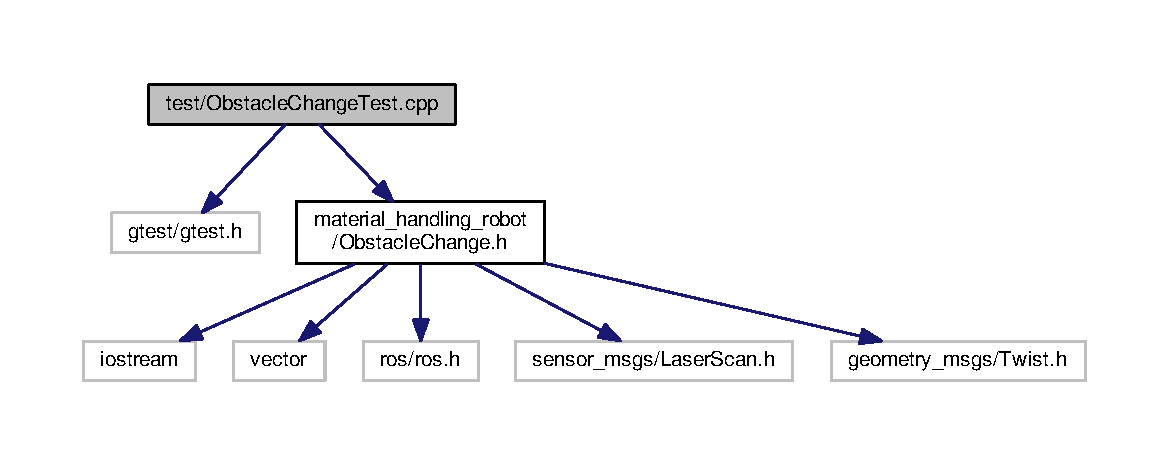
\includegraphics[width=350pt]{ObstacleChangeTest_8cpp__incl}
\end{center}
\end{figure}
\subsection*{Functions}
\begin{DoxyCompactItemize}
\item 
\hyperlink{ObstacleChangeTest_8cpp_afc89f59b31b71b0f6af9bca3955bff4a}{T\+E\+ST} (Obstacle\+Change\+Test, set\+Target\+Point\+Test)
\begin{DoxyCompactList}\small\item\em Test function to test the string conversion. \end{DoxyCompactList}\item 
\hyperlink{ObstacleChangeTest_8cpp_a6ff32f330ff66346c080b8e21c635e1d}{T\+E\+ST} (Obstacle\+Change\+Test, spawn\+Object\+Test)
\begin{DoxyCompactList}\small\item\em Test function to test the object spawn function. \end{DoxyCompactList}\item 
\hyperlink{ObstacleChangeTest_8cpp_ac7b22eca26e3e33e20794df42064c736}{T\+E\+ST} (Object\+Manipulation\+Test, destroy\+Object\+Test)
\begin{DoxyCompactList}\small\item\em Test function for removing the object. \end{DoxyCompactList}\end{DoxyCompactItemize}


\subsection{Detailed Description}
Tests the member methods of \hyperlink{classObstacleChange}{Obstacle\+Change} class. 

M\+IT License

Copyright (c) 2019 Vamshi Bogoju, Raja Srinivas Iskala

Permission is hereby granted, free of charge, to any person obtaining a copy of this software and associated documentation files (the \char`\"{}\+Software\char`\"{}), to deal in the Software without restriction, including without limitation the rights to use, copy, modify, merge, publish, distribute, sublicense, and/or sell copies of the Software, and to permit persons to whom the Software is furnished to do so, subject to the following conditions\+:

The above copyright notice and this permission notice shall be included in all copies or substantial portions of the Software.

T\+HE S\+O\+F\+T\+W\+A\+RE IS P\+R\+O\+V\+I\+D\+ED \char`\"{}\+A\+S I\+S\char`\"{}, W\+I\+T\+H\+O\+UT W\+A\+R\+R\+A\+N\+TY OF A\+NY K\+I\+ND, E\+X\+P\+R\+E\+SS OR I\+M\+P\+L\+I\+ED, I\+N\+C\+L\+U\+D\+I\+NG B\+UT N\+OT L\+I\+M\+I\+T\+ED TO T\+HE W\+A\+R\+R\+A\+N\+T\+I\+ES OF M\+E\+R\+C\+H\+A\+N\+T\+A\+B\+I\+L\+I\+TY, F\+I\+T\+N\+E\+SS F\+OR A P\+A\+R\+T\+I\+C\+U\+L\+AR P\+U\+R\+P\+O\+SE A\+ND N\+O\+N\+I\+N\+F\+R\+I\+N\+G\+E\+M\+E\+NT. IN NO E\+V\+E\+NT S\+H\+A\+LL T\+HE A\+U\+T\+H\+O\+RS OR C\+O\+P\+Y\+R\+I\+G\+HT H\+O\+L\+D\+E\+RS BE L\+I\+A\+B\+LE F\+OR A\+NY C\+L\+A\+IM, D\+A\+M\+A\+G\+ES OR O\+T\+H\+ER L\+I\+A\+B\+I\+L\+I\+TY, W\+H\+E\+T\+H\+ER IN AN A\+C\+T\+I\+ON OF C\+O\+N\+T\+R\+A\+CT, T\+O\+RT OR O\+T\+H\+E\+R\+W\+I\+SE, A\+R\+I\+S\+I\+NG F\+R\+OM, O\+UT OF OR IN C\+O\+N\+N\+E\+C\+T\+I\+ON W\+I\+TH T\+HE S\+O\+F\+T\+W\+A\+RE OR T\+HE U\+SE OR O\+T\+H\+ER D\+E\+A\+L\+I\+N\+GS IN T\+HE S\+O\+F\+T\+W\+A\+RE. \begin{DoxyCopyright}{Copyright}
2019 

M\+IT License
\end{DoxyCopyright}
Design (iteration 1) \begin{DoxyAuthor}{Author}
Vamshi -\/ Navigator 

Raja -\/ Driver  (iteration 3) 

Vamshi -\/ Driver 

Raja -\/ Navigator 
\end{DoxyAuthor}
\begin{DoxyDate}{Date}
4/12/2019 
\end{DoxyDate}
\begin{DoxyVersion}{Version}
1.\+0 
\end{DoxyVersion}


\subsection{Function Documentation}
\index{Obstacle\+Change\+Test.\+cpp@{Obstacle\+Change\+Test.\+cpp}!T\+E\+ST@{T\+E\+ST}}
\index{T\+E\+ST@{T\+E\+ST}!Obstacle\+Change\+Test.\+cpp@{Obstacle\+Change\+Test.\+cpp}}
\subsubsection[{\texorpdfstring{T\+E\+S\+T(\+Obstacle\+Change\+Test, set\+Target\+Point\+Test)}{TEST(ObstacleChangeTest, setTargetPointTest)}}]{\setlength{\rightskip}{0pt plus 5cm}T\+E\+ST (
\begin{DoxyParamCaption}
\item[{Obstacle\+Change\+Test}]{, }
\item[{set\+Target\+Point\+Test}]{}
\end{DoxyParamCaption}
)}\hypertarget{ObstacleChangeTest_8cpp_afc89f59b31b71b0f6af9bca3955bff4a}{}\label{ObstacleChangeTest_8cpp_afc89f59b31b71b0f6af9bca3955bff4a}


Test function to test the string conversion. 


\begin{DoxyParams}{Parameters}
{\em Obstacle\+Change\+Test} & gtest framework \\
\hline
{\em set\+Target\+Point\+Test} & name of test \\
\hline
\end{DoxyParams}
\begin{DoxyReturn}{Returns}
None 
\end{DoxyReturn}
\index{Obstacle\+Change\+Test.\+cpp@{Obstacle\+Change\+Test.\+cpp}!T\+E\+ST@{T\+E\+ST}}
\index{T\+E\+ST@{T\+E\+ST}!Obstacle\+Change\+Test.\+cpp@{Obstacle\+Change\+Test.\+cpp}}
\subsubsection[{\texorpdfstring{T\+E\+S\+T(\+Obstacle\+Change\+Test, spawn\+Object\+Test)}{TEST(ObstacleChangeTest, spawnObjectTest)}}]{\setlength{\rightskip}{0pt plus 5cm}T\+E\+ST (
\begin{DoxyParamCaption}
\item[{Obstacle\+Change\+Test}]{, }
\item[{spawn\+Object\+Test}]{}
\end{DoxyParamCaption}
)}\hypertarget{ObstacleChangeTest_8cpp_a6ff32f330ff66346c080b8e21c635e1d}{}\label{ObstacleChangeTest_8cpp_a6ff32f330ff66346c080b8e21c635e1d}


Test function to test the object spawn function. 


\begin{DoxyParams}{Parameters}
{\em Obstacle\+Change\+Test} & gtest framework \\
\hline
{\em spawn\+Object\+Test} & name of test \\
\hline
\end{DoxyParams}
\begin{DoxyReturn}{Returns}
None 
\end{DoxyReturn}
\index{Obstacle\+Change\+Test.\+cpp@{Obstacle\+Change\+Test.\+cpp}!T\+E\+ST@{T\+E\+ST}}
\index{T\+E\+ST@{T\+E\+ST}!Obstacle\+Change\+Test.\+cpp@{Obstacle\+Change\+Test.\+cpp}}
\subsubsection[{\texorpdfstring{T\+E\+S\+T(\+Object\+Manipulation\+Test, destroy\+Object\+Test)}{TEST(ObjectManipulationTest, destroyObjectTest)}}]{\setlength{\rightskip}{0pt plus 5cm}T\+E\+ST (
\begin{DoxyParamCaption}
\item[{Object\+Manipulation\+Test}]{, }
\item[{destroy\+Object\+Test}]{}
\end{DoxyParamCaption}
)}\hypertarget{ObstacleChangeTest_8cpp_ac7b22eca26e3e33e20794df42064c736}{}\label{ObstacleChangeTest_8cpp_ac7b22eca26e3e33e20794df42064c736}


Test function for removing the object. 


\begin{DoxyParams}{Parameters}
{\em Obstacle\+Change\+Test} & gtest framework \\
\hline
{\em destroy\+Object\+Test} & name of test \\
\hline
\end{DoxyParams}
\begin{DoxyReturn}{Returns}
None 
\end{DoxyReturn}

%--- End generated contents ---

% Index
\backmatter
\newpage
\phantomsection
\clearemptydoublepage
\addcontentsline{toc}{chapter}{Index}
\printindex

\end{document}
